% $Id%

% ++++++++++++++++++++++++++++++++++++++++++++++++++++++++++++++++++++++++++
%\newpage  be_2006 N�tig ?
\hypertarget{appendix-start}{}\label{s:appendix-start}
% \addcontentsline{toc}{section}{Anhang} 
% \addcontentsline macht nur Eintrag ins Inhaltsverzeichnis und deren PDF-Darstellung im linken Frame (mit den Kapitel�berschriften). 
%be_2005: Arbeitet man hier mit \addcontentsline{toc}{section}{Anhang} und man
%         nutzt statt \section das \subsection, damit es korrekterweise
%         unterhalb von Appendix einetragen wird, hat es das Pr�fix ".1" oder ".2"
%         statt �" oder "B".
% --> L�sung: nur section (da der Link im Content vorher immer eine Seite zu fr�h ansprang)

\section{Anhang}

    \begin{itemize}

      \item[1] \hyperlink{appendix-menutree}{CrypTool Men�baum}

      \item[2] \hyperlink{appendix-authors}{Autoren des CrypTool-Skripts}

      \item[3] \hyperlink{appendix-movies}{Filme und belletristische
                          Literatur mit Bezug zur Kryptographie, B�cher
                          mit Sammlungen einfacher Verfahren f�r Kinder}

      \item[4] \hyperlink{appendix-Learn-NT}
                         {Lernprogramm Elementare Zahlentheorie}
    \end{itemize}




% ++++++++++++++++++++++++++++++++++++++++++++++++++++++++++++++++++++++++++
\newpage
\enlargethispage{1cm}
\hypertarget{appendix-menutree}{}
\subsection{CrypTool-Men�s}
\label{s:appendix-menutree}

   % Eyecatcher_Neue-CrypTool-Version
Dieser Anhang enth�lt auf der folgenden Seite den kompletten Men�-Baum der
CrypTool\index{CrypTool}-Version 1.4.10.

Welche Men�eintr�ge gerade aktiv (also nicht ausgegraut) sind, wird durch
den Typ des aktiven Dokumentenfenster bestimmt.

So ist z.~B. die Brute-Force Analyse\index{Angriff!Brute-force} f�r DES 
nur verf�gbar, wenn das aktive Fenster in Hexadezi"-mal-Darstellung 
ge�ffnet ist, w�hrend der Men�eintrag "`Zufallsdaten erzeugen\dots"'
immer verf�gbar ist (auch wenn kein Dokument ge�ffnet ist). 

%Folgende vier Dokumenttypen gibt es in CrypTool:
%\begin{center}
%\begin{tabular}{rl}
%\bf Codebuchstabe & \bf Dokumententyp \\
%T & Textdatei-Ansicht\\
%H & Hexadezimal-Ansicht\\
%P & Diagramm/Plot-Ansicht (Histogramm, Autokorrelation)\\
%O & OpenGL Graphics-Ansicht\\
%\end{tabular}
%\end{center}


\clearpage
\begin{figure}[hb]
\begin{center}
\vspace{-30pt}
%\frame{
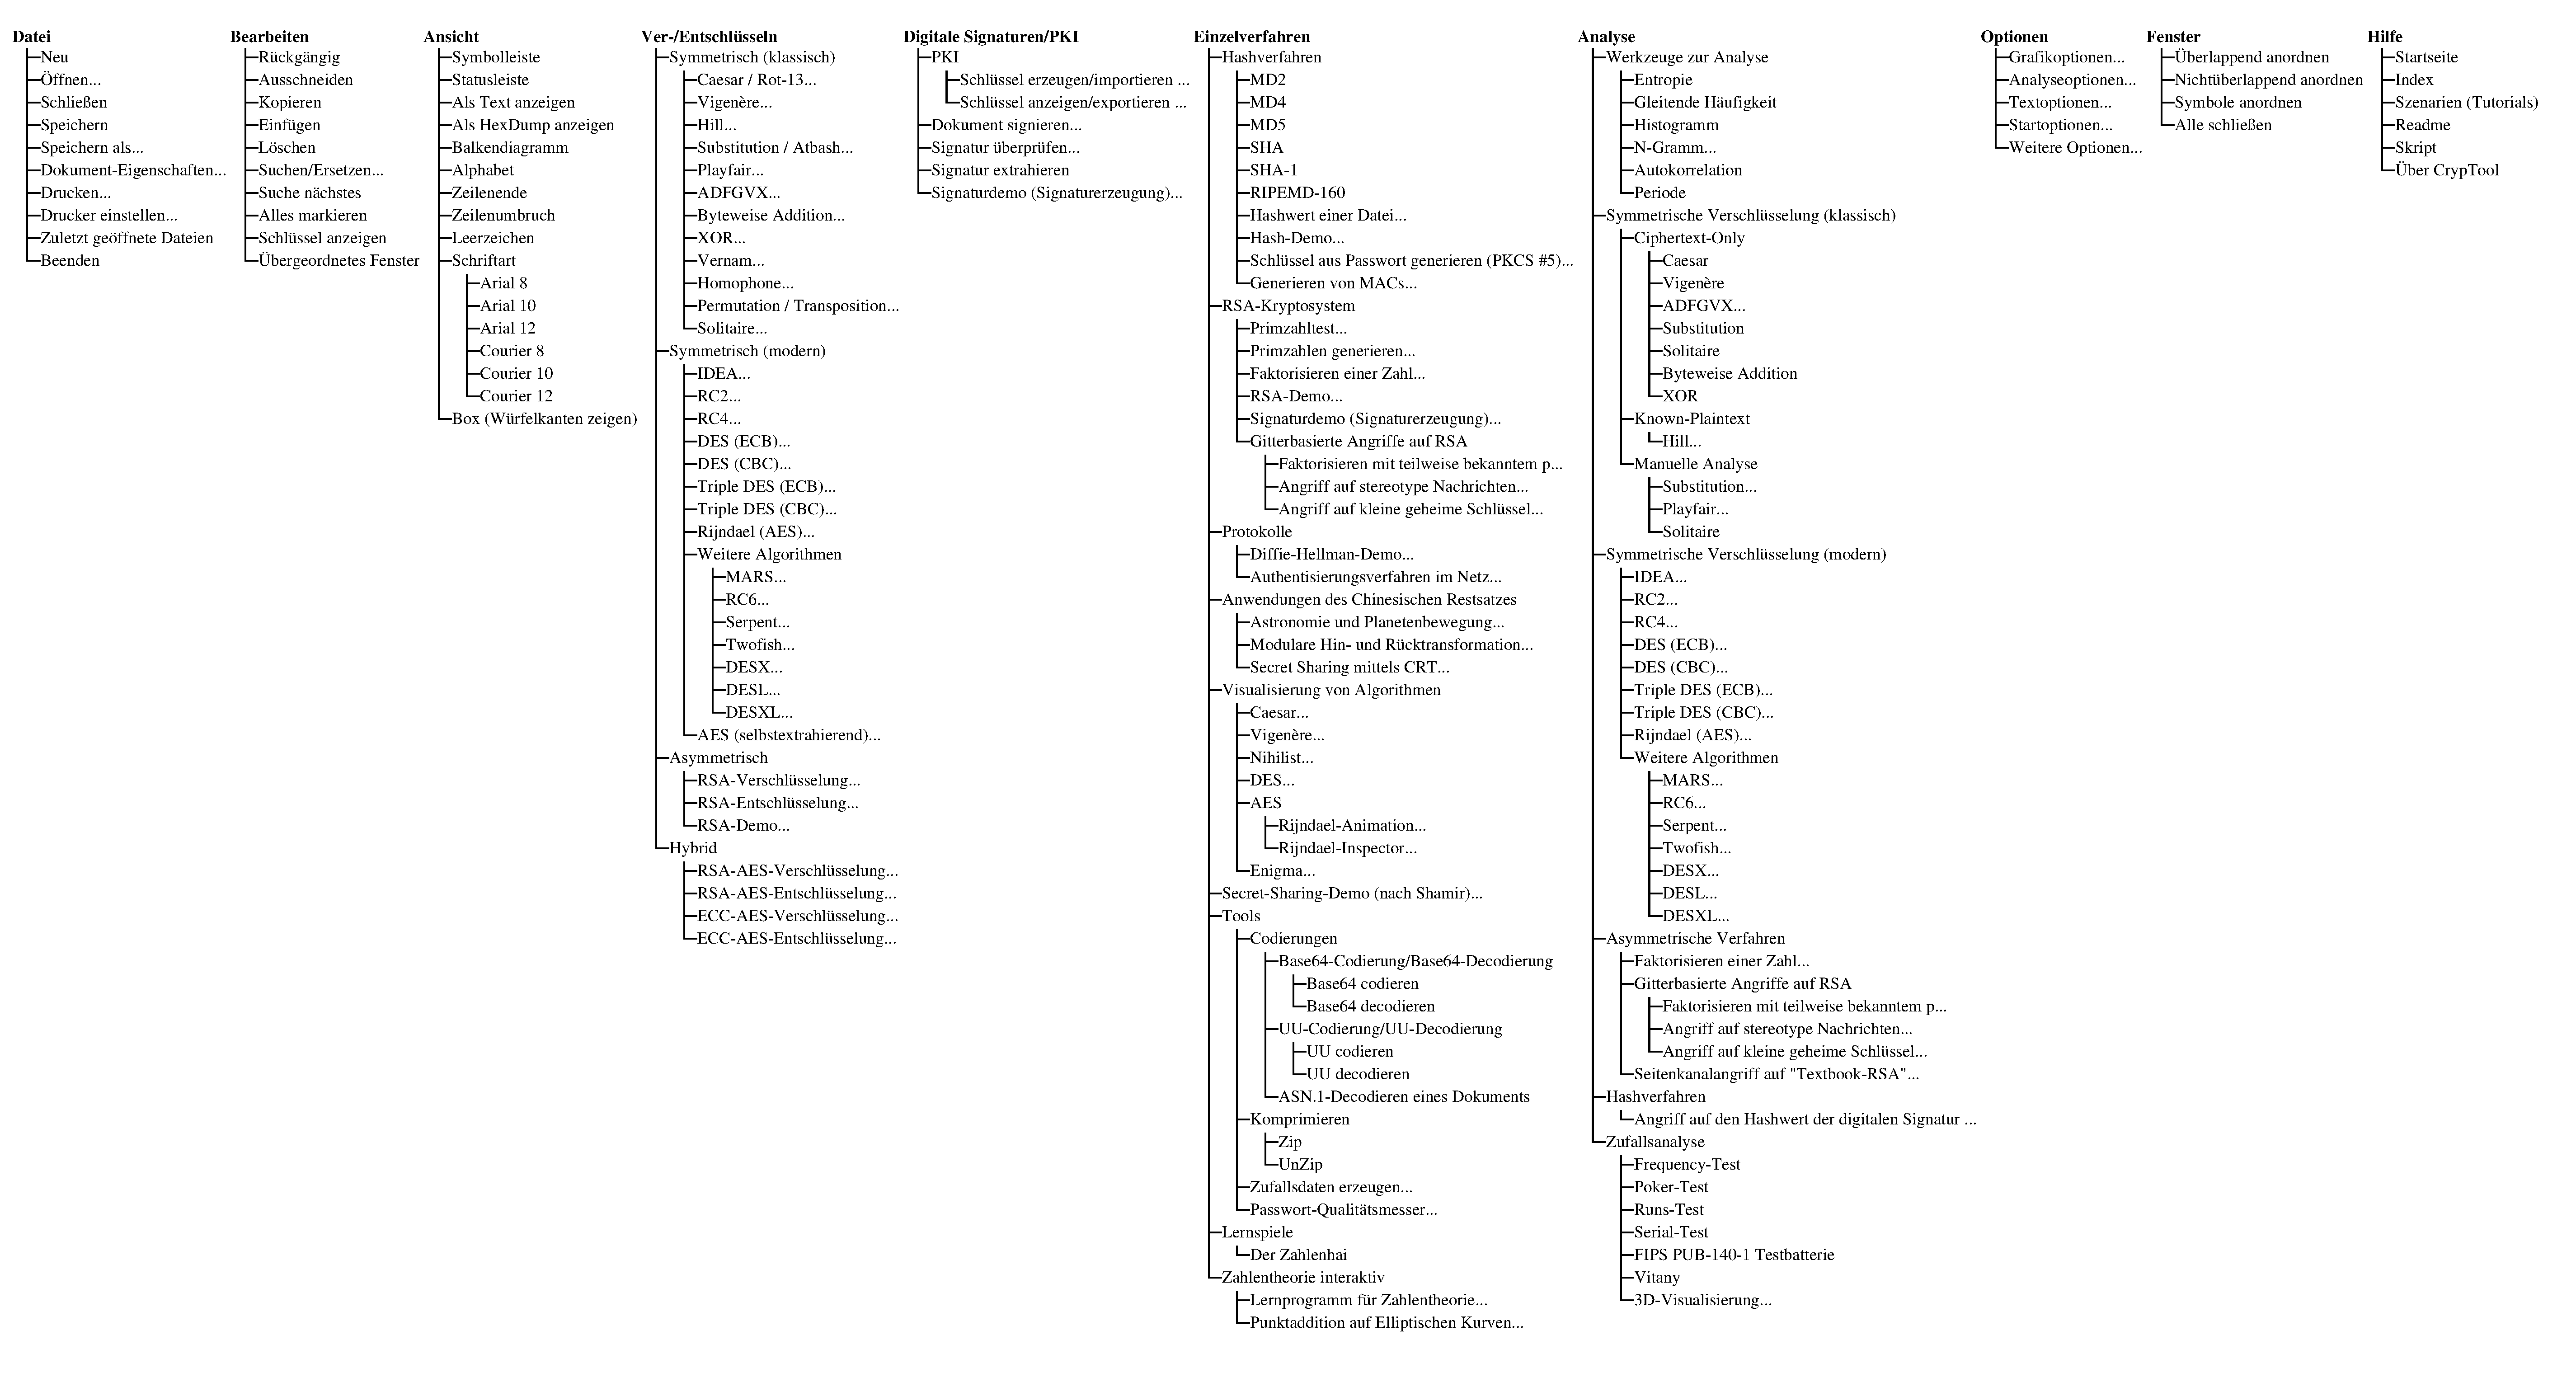
\includegraphics[scale=0.25, angle=270, viewport=200 3 2680 1276]
                {figures/cryptool-menu-de}
%viewport=rand-links? rand-unten breite hoehe? [bezogen auf querformat]
%}
\caption{Komplette �bersicht �ber den Men�-Baum von CrypTool 1.4.10} 
\label{menuoverview}
\end{center}
\end{figure}
\clearpage

